Auf modernen CCD- oder CMOS-Bildsensoren werden oft sogenannte Microlenses
verwendet.
Dies sind kleine Linsen, die direkt auf dem Chip aufgebracht sind und
das Licht auf die lichtempfindlichen Fotodioden fokusieren.
Dadurch wird es möglich, auch das Licht zu nutzen, welches ohne diese
Microlenses auf die von Elektroden abgedeckten 
Flächen fallen würde, und so die Empfindlichkeit zu steigern.
Je nach Konstruktion der Microlenses kann erreicht werden, dass fast
100\% des einfallenden Lichts genutzt werden kann
(Abbildung~\ref{10000061:fig1}).
\begin{figure}[ht]
\centering
\includeagraphics[width=0.4\hsize]{microlensarray.jpg}
\qquad
\includeagraphics[width=0.4\hsize]{photodiode.jpg}
\caption{Ein Microlens-Array kann die Lichtausbeute eines CCD-Chips
verbessern.
\label{10000061:fig1}}
\end{figure}

Betrachten Sie jetzt einen Microlens-Array aus kugelförmigen Microlenses
aus einem Material mit dem Brechungsindex $n=1.5=\frac32$.
Der Radius der gekrümmten Fläche sei $r=10\,\mu\text{m}$.
Der Einfachheit halber betrachten wir jetzt Licht, welches senkrecht
auf den Microlens-Array einfällt.
Wie dick muss der Microlens-Array sein, damit das Licht auf der
Sensorfläche fokusiert wird?

\begin{hinweis}
Rechnen Sie in paraxialer Näherung.
\end{hinweis}

\thema{Matrixoptik}

\begin{figure}[h]
\centering
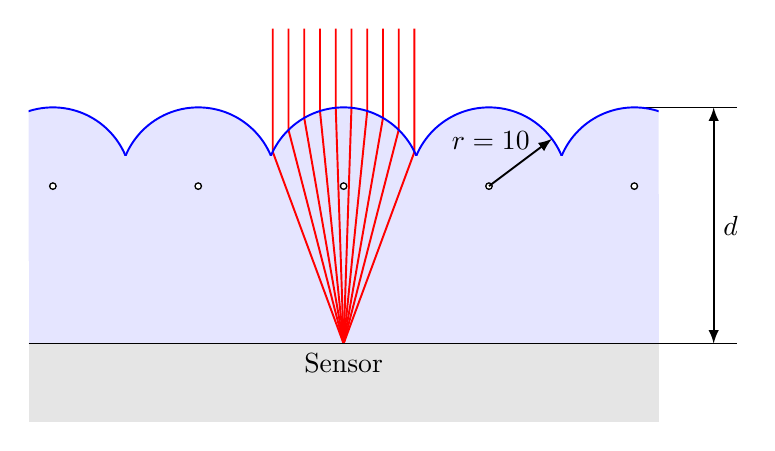
\begin{tikzpicture}[>=latex]

\def\d{12/13}
\def\h{5/13}
\begin{scope}
\clip (-4,-1) rectangle (4,2);
\foreach \x in {-6,-4,...,6}{
	\fill[color=blue!10] ({\x*\d},0) circle[radius=1];
	\fill ({\x*\d},0) circle[radius=0.05];
	\fill[color=white] ({\x*\d},0) circle[radius=0.03];
}
\end{scope}

\fill[color=blue!10] (-4,-2) rectangle (4,-0.1);

\foreach \x in {-0.9,-0.7,...,0.9}{
	\draw[color=red,line width=0.7pt] (\x,2)--(\x,{sqrt(1-\x*\x)})--(0,-2);
}

\draw[line width=0.2pt] (4,-2)--(5,-2);
\draw[line width=0.2pt] ({4*\d},1)--(5,1);
\draw[<->,line width=0.7pt] (4.7,-2)--(4.7,1);
\node at (4.7,-0.5) [right] {$d$};

\draw[line width=0.7pt] (-4,-2)--(4,-2);
\fill[color=gray!20] (-4,-3) rectangle (4,-2);
\node at (0,-2) [below] {Sensor};

\begin{scope}
\clip (-4,{\h}) rectangle (4,2);
\foreach \x in {-6,-4,...,6}{
	\draw[color=blue,line width=0.7pt] ({\x*\d},0) circle[radius=1];
}
\end{scope}
\draw[line width=0.7pt,->] ({2*\d},0)--({2*\d+0.8},0.6);
\node at ({2*\d+0.8*0.8},0.6*0.8+0.1) [left] {$r=10$};

\end{tikzpicture}
\caption{Lichtbrechung an einem Microlens-Array
\label{10000061:fig}}
\end{figure}


\begin{loesung}
Die Wirkung der Oberfläche der Microlens wird durch die Matrix
\[
T_o
=
B(1,n,r)
=
B(1,{\textstyle\frac32},10)
=
\begin{pmatrix}1&0\\(\frac{1}{n}-1)/r&\frac1n\end{pmatrix}
=
\begin{pmatrix}1&0\\(\frac{2}{3}-1)/r&\frac23\end{pmatrix}
=
\begin{pmatrix}1&0\\-\frac{1}{30}&\frac23\end{pmatrix}
\]
beschrieben.
Hat der Microlens-Array die Dicke $d$, dann können wir die Gesamtwirkung
des Arrays aus dem Matrizenprodukt
\[
T
=
T_d
T_o
=
\begin{pmatrix}1&d\\0&1\end{pmatrix}
\begin{pmatrix}1&0\\-\frac{1}{30}&\frac23\end{pmatrix}
=
\begin{pmatrix}
1-\frac{d}{30} & \frac{2d}{3} \\
-\frac1{30} & \frac23
\end{pmatrix}
\]
erhalten.
Parallel einfallende Strahlen haben verschwindende zweite Komponente,
gesucht ist dann derjenige Wert von $d$, für den die erste Komponente
von $Te_1$ verschwindet.
Es ist
\begin{align*}
Te_1
&=
\begin{pmatrix}
1-\frac{d}{30} & \frac{2d}{3} \\
-\frac1{30} & \frac23
\end{pmatrix}
\begin{pmatrix}1\\0\end{pmatrix}
=
\begin{pmatrix}
1-\frac{d}{30} \\
-\frac1{30} 
\end{pmatrix}.
\end{align*}
Die erste Komponenten verschwindet genau dann, wenn 
\[
1-\frac{d}{30} = 0
\qquad\Leftrightarrow\qquad
d=30
\]
ist.
Der Microlens-Array muss also $d=30\,\mu\text{m}$ dick sein.
\end{loesung}

\begin{bewertung}
Matrix $T_d$ ({\bf T}) 1 Punkt,
Matrix $T_o$ ({\bf O}) 1 Punkt,
Eingangsvektor ({\bf E}) 1 Punkt,
Ausgangsvektor ({\bf V}) 1 Punkt,
Gleichung für Abstand ({\bf G}) 1 Punkt,
Abstand ({\bf D}) 1 Punkt.
\end{bewertung}
